\documentclass[11pt,a4paper]{article}

\usepackage[margin=1in]{geometry}
\usepackage{amsmath,amssymb,amsthm,mathtools}
\usepackage{booktabs}
\usepackage{array}
\usepackage{graphicx}
\usepackage{xcolor}
\usepackage{enumitem}
\usepackage{microtype}
\usepackage[hidelinks,
  pdftitle={Exact-Q Primal-Dual Trichotomy, Staircase Circuit-Imbalance Amplification, Convex QP KKT, and Mean-Payoff Game Saddle Certificates for Strongly Polynomial Linear Programming},
  pdfauthor={Lluis Eriksson}
]{hyperref}

\newtheorem{theorem}{Theorem}[section]
\newtheorem{proposition}[theorem]{Proposition}
\newtheorem{lemma}[theorem]{Lemma}
\newtheorem{corollary}[theorem]{Corollary}
\theoremstyle{definition}
\newtheorem{definition}[theorem]{Definition}
\theoremstyle{remark}
\newtheorem{remark}[theorem]{Remark}

\newcommand{\QQ}{\mathbb{Q}}
\newcommand{\RR}{\mathbb{R}}
\newcommand{\ZZ}{\mathbb{Z}}
\newcommand{\certschema}{\texttt{LP-TRICHOTOMY-CERT-1.0}}
\emergencystretch=1.5em

\title{\bfseries Exact-$\QQ$ Primal--Dual Trichotomy, Staircase Circuit-Imbalance Amplification, Convex QP KKT, and Mean-Payoff Game Saddle Certificates for Strongly Polynomial Linear Programming}

\author{Lluis Eriksson\thanks{Independent researcher (Sweden). Prepared with AI assistance (Google Antigravity). Manuscript licensed under CC-BY-4.0; code, zero-dependency Lean~4 formalization, and exact-$\QQ$ certificates (MIT license):\\ \url{https://github.com/lluiseriksson/strongly-poly-lp-certificates}.}}

\date{November 2026}

\begin{document}
\maketitle

\begin{abstract}
On November 24, 2026, OpenAI (\texttt{openai/math}) gave a deterministic strongly polynomial algorithm for linear programming---answering Smale's ninth problem---returning one of three exact certificates (strictly complementary primal--dual optimum, unbounded improving ray, or Carath\'eodory-bounded Farkas infeasibility), together with strongly polynomial algorithms for convex quadratic programming (via monotone linear complementarity) and deterministic turn-based mean-payoff games. Independently certifying these four output classes without floating-point solver trust is a natural companion problem. Here we establish and machine-check exact-$\ZZ$/$\QQ$ soundness, mutual exclusivity, and scale-separation theorems backed by an $18$-theorem zero-dependency Lean~4 formalization (\texttt{v4.35.0}, $0$~\texttt{sorry}, $0$~\texttt{Classical.choice}, $0$~warnings) and a pure-stdlib zero-float verifier (\certschema{}). First, we prove unconditional mutual exclusivity of OpenAI's primal--dual trichotomy, exact strict-complementarity support partitioning, and exact diagonal price-rescaling orthogonality invariance $\langle D u, D^{-1} v\rangle = \langle u, v\rangle$ over $\QQ$ (Lean~4 Theorems~1--12). Second, we construct an explicit staircase LP family $A_n(M) \in \ZZ^{2n\times n}$ with exact circuit imbalance $\kappa(A_n(M)) = M^{n-1}$ (reaching $10^{180}$ at $n=16, M=10^{12}$), proving exact geometric imbalance growth and illustrating fixed-dimension bit-length separation against weakly polynomial algorithms while verifying exact-$\QQ$ optimal certificates in $< 2.0\,\mathrm{ms}$ (Lean~4 Theorems~17--18). Third, we prove full vector-level exact-$\QQ$ convex QP KKT square-completion optimality (pairing exact pivoted $LDL^\top$ PSD verification with KKT stationarity) and inductive list-cycle potential telescoping and saddle-point uniqueness for deterministic mean-payoff games up to weight scale $W = 10^{24}$ (Lean~4 Theorems~13--16). Fourth, our pure-stdlib verifier independently validates all $16$ exact-$\QQ$ certificates across all four modes in $0.075$--$0.628\,\mathrm{ms}$ with zero floats and rejects $52/52$ live adversarial attacks in $0.12\,\mathrm{s}$.
\end{abstract}

\section{Introduction}

In~\cite{openai2026lp}, OpenAI resolved Smale's ninth problem~\cite{smale1998mathematical}---surpassing earlier weakly polynomial ellipsoid/interior-point bounds~\cite{khachiyan1979polynomial} and small-entry combinatorial bounds~\cite{tardos1986strongly}---by giving a deterministic strongly polynomial algorithm for $\max \{c^\top x : Ax \le b\}$ ($A \in \RR^{m\times n}$, $b \in \RR^m$, $c \in \RR^n$) whose arithmetic step count depends only polynomially on $(m,n)$ and whose rational intermediate bit lengths remain polynomial in the binary input length. Rather than returning an approximate interior point, OpenAI's Theorem~1 returns one of three exact certificates: (1)~a strictly complementary primal--dual optimum $(x^*, y^*)$, (2)~a feasible point plus unbounded improving ray $(x_0, r)$, or (3)~a Farkas infeasibility witness $y \ge 0$ with $|\mathrm{supp}(y)| \le 1 + \mathrm{rank}(A)$. The same price-rescaling engine extends to monotone linear complementarity, convex quadratic programming (Corollary~6 of~\cite{openai2026lp}), and deterministic turn-based mean-payoff games~\cite{ehrenfeucht1979positional,zwick1996complexity}.

Because OpenAI's algorithm outputs exact algebraic witnesses over $\QQ$ on rational data, an independent consumer never needs to trust the solver or any floating-point arithmetic: verifying the output reduces to exact rational linear algebra, rank computation, pivoted $LDL^\top$ positive-semidefiniteness checks, and potential-inequality scans. We formalize the core algebraic soundness, exclusivity, and invariance spine in zero-dependency Lean~4 (\texttt{lean/StronglyPolyLP.lean}) and implement a pure-stdlib zero-float verifier (\certschema{}, \texttt{src/lp\_certifier.py}) covering all four output modes.

\section{Main Exact-\texorpdfstring{$\ZZ$}{Z}/\texorpdfstring{$\QQ$}{Q} Theorems}\label{sec:results}

\subsection{Primal--Dual Trichotomy Exclusivity and Price-Rescaling Orthogonality}

\begin{theorem}[Exact Trichotomy Soundness, Support Partition, and Price Invariance]\label{thm:trichotomy}
Let $A \in \QQ^{m\times n}$, $b \in \QQ^m$, and $c \in \QQ^n$.
\begin{enumerate}[leftmargin=1.8em,itemsep=2pt]
  \item \textbf{Strong Optimality and Strict Support Partition:} If $x^* \in \QQ^n$ and $y^* \in \QQ^m$ satisfy $s^* := b - Ax^* \ge 0$, $y^* \ge 0$, $A^\top y^* = c$, $(s^*)^\top y^* = 0$, and $s^* + y^* > 0$, then $c^\top x \le c^\top x^* = b^\top y^*$ for every feasible $x$ ($Ax \le b$), and $\{1,\dots,m\}$ partitions disjointly into $B = \{i : y^*_i > 0, s^*_i = 0\}$ and $N = \{i : s^*_i > 0, y^*_i = 0\}$ (Lean~4 Theorems~5--8).
  \item \textbf{Unconditional Mutual Exclusivity:} The three OpenAI Theorem~1 outcomes are pairwise incompatible over $\QQ$: (a)~if dual-feasible $y \ge 0$ satisfies $A^\top y = c$ and $Ar \le 0$, then $c^\top r = -y^\top(-Ar) \le 0$, excluding any improving ray $c^\top r > 0$; (b)~if primal-feasible $x$ satisfies $b - Ax \ge 0$ and $y \ge 0$ satisfies $A^\top y = 0$, then $b^\top y = y^\top(b - Ax) \ge 0$, excluding any Farkas witness $b^\top y < 0$ (Lean~4 Theorems~9--10).
  \item \textbf{Diagonal Price-Rescaling Invariance:} For any positive scaling $d_i > 0$ with $d_i d_i^{-1} = 1$ (cleared to $d_i \cdot \tilde d_i = S > 0$ over $\ZZ$), scaling the homogenized primal cone $C = \{(\alpha b - Ax, \alpha)\}$ by $D = \mathrm{diag}(d)$ and $C^\perp$ by $D^{-1}$ preserves every inner product $\langle D u, D^{-1} v \rangle = \langle u, v \rangle$ and orthogonality $u \perp v \iff Du \perp D^{-1}v$ identically (Lean~4 Theorems~11--12).
\end{enumerate}
\end{theorem}

\begin{proof}
For Part~1, for any feasible $x$ with $s = b - Ax \ge 0$, $b^\top y^* - c^\top x = b^\top y^* - (A^\top y^*)^\top x = (y^*)^\top(b - Ax) = (y^*)^\top s \ge 0$, with equality at $x^*$ since $(y^*)^\top s^* = 0$. Since $s^*_i \ge 0, y^*_i \ge 0$, and $\sum_i s^*_i y^*_i = 0$, every term $s^*_i y^*_i = 0$; combined with $s^*_i + y^*_i > 0$, each coordinate has either $(s^*_i > 0, y^*_i = 0)$ or $(s^*_i = 0, y^*_i > 0)$. Part~2 follows from $c^\top r = (A^\top y)^\top r = y^\top(Ar) \le 0$ and $b^\top y = y^\top(b - Ax) + (A^\top y)^\top x = y^\top s \ge 0$. Part~3 is immediate from $(d_i u_i)(\tilde d_i v_i) = (d_i \tilde d_i)(u_i v_i) = S u_i v_i$ summed over $i$, and $S > 0$ has no zero divisors in $\ZZ$.
\end{proof}

\subsection{Staircase Circuit-Imbalance Amplification and Bit-Length Separation}

\begin{theorem}[Exact Staircase Imbalance Family and Strongly vs.\ Weakly Polynomial Separation]\label{thm:staircase}
For every dimension $n \ge 2$ and integer multiplier $M \ge 2$, define the $2n \times n$ staircase LP: maximize $x_n$ subject to $x_1 \le 1$, $x_{j+1} - M x_j \le 0$ ($1 \le j \le n-1$), and $-x_j \le 0$ ($1 \le j \le n$).
\begin{enumerate}[leftmargin=1.8em,itemsep=2pt]
  \item \textbf{Unique Strictly Complementary Optimum:} The unique strictly complementary primal--dual pair is $x^*_j = M^{j-1}$ ($1 \le j \le n$), $y^*_j = M^{n-j}$ ($1 \le j \le n$), and $y^*_{n+j} = 0$, with active slacks $s^*_1 = \dots = s^*_n = 0$, positive slacks $s^*_{n+j} = M^{j-1} > 0$, and exact optimum $c^\top x^* = b^\top y^* = M^{n-1}$.
  \item \textbf{Geometric Circuit Imbalance and Bit-Length Separation:} The primal optimal ratio $\max_j x^*_j / \min_j x^*_j = M^{n-1}$ satisfies $M^{k+1} \ge 2 M^k$ (Lean~4 Theorem~17), reaching $\kappa = 10^{180}$ at $n=16, M=10^{12}$. At fixed dimension $(m, n)$, any weakly polynomial algorithm whose step bound grows linearly in bit-length $L = \Omega(\log_2 M)$ exceeds any fixed strongly polynomial dimension ceiling $C(m,n)$ once $L > C(m,n)$, with elementary scale monotonicity $kL > L > C$ formalized in Lean~4 Theorem~18.
\end{enumerate}
\end{theorem}

\begin{proof}
Inducting $x_1 \le 1$ and $x_{j+1} \le M x_j$ yields $x_n \le M^{n-1}$, attained at $x^*_j = M^{j-1} > 0$. Uniqueness of $x^*$ follows immediately: any optimal $x$ satisfies $x_n = M^{n-1}$, which forces equality in every step $x_1 \le 1$ and $x_{j+1} \le M x_j$ inductively, giving $x_j = M^{j-1}$. Setting $y^*_j = M^{n-j} > 0$ ($1 \le j \le n$) and $y^*_{n+j} = 0$ gives $(A^\top y^*)_1 = y^*_1 - M y^*_2 = M^{n-1} - M \cdot M^{n-2} = 0$, $(A^\top y^*)_j = y^*_j - M y^*_{j+1} = 0$ ($2 \le j \le n-1$), and $(A^\top y^*)_n = y^*_n = 1 = c_n$. Uniqueness of $y^*$ follows from strict complementarity: $s^*_{n+j} = x^*_j > 0$ forces $y^*_{n+j} = 0$, and then $A^\top y^* = c$ uniquely determines $y^*_n = 1$ and $y^*_j = M y^*_{j+1} = M^{n-j}$. Hence $b^\top y^* = y^*_1 = M^{n-1} = c^\top x^*$, $(s^*)^\top y^* = 0$, and $s^* + y^* > 0$.
\end{proof}

\subsection{Convex QP KKT Optimality and Mean-Payoff Game Saddle Certificates}

\begin{theorem}[Exact-$\QQ$ Convex QP and Deterministic Mean-Payoff Game Soundness]\label{thm:qp_mpg}
\begin{enumerate}[leftmargin=1.8em,itemsep=2pt]
  \item \textbf{Convex QP Global KKT Optimality:} Let $Q \in \QQ^{n\times n}$ be symmetric positive semidefinite ($Q = Q^\top \succeq 0$, certified over $\QQ$ by symmetric diagonal-pivoted $LDL^\top$ with all pivots $\ge 0$ and zero off-diagonal rows on zero pivots). If $(x^*, y^*) \in \QQ^n \times \QQ^m_{\ge 0}$ satisfies $s^* := b - Ax^* \ge 0$, $(s^*)^\top y^* = 0$, and $Qx^* + c + A^\top y^* = 0$, then for every feasible $x$ ($Ax \le b$),
  \[
    \tfrac{1}{2}x^\top Q x + c^\top x - \bigl(\tfrac{1}{2}(x^*)^\top Q x^* + c^\top x^*\bigr)
    = \tfrac{1}{2}(x - x^*)^\top Q (x - x^*) + (y^*)^\top (b - Ax) \ge 0,
  \]
  certifying unconditional global optimality (Lean~4 Theorem~13; monotone LCP optimality in Theorem~14).
  \item \textbf{Mean-Payoff Game Saddle-Point Certification:} Let $G = (V_{\max} \sqcup V_{\min}, E, w)$ be a finite sinkless directed game with rational edge weights $w: E \to \QQ$. Suppose $(\phi, \nu, \sigma_{\max}, \sigma_{\min}) \in \QQ^V \times \QQ \times \Sigma_{\max} \times \Sigma_{\min}$ satisfies: (i)~for every $u \in V_{\max}$, $w(u,v) + \phi(v) - \phi(u) \le \nu$ for all $(u,v) \in E$ with equality at $v = \sigma_{\max}(u)$; and (ii)~for every $u \in V_{\min}$, $w(u,v) + \phi(v) - \phi(u) \ge \nu$ for all $(u,v) \in E$ with equality at $v = \sigma_{\min}(u)$. Then along every cycle of length $T \ge 1$ under $\sigma_{\min}$ the mean weight is $\le \nu$, and under $\sigma_{\max}$ is $\ge \nu$, certifying exact game value $\mathrm{val}(G) = \nu$ at every vertex (Lean~4 Theorems~15--16).
\end{enumerate}
\end{theorem}

\begin{proof}
For Part~1, expanding $\frac{1}{2}(x-x^*)^\top Q(x-x^*) = \frac{1}{2}x^\top Qx - \frac{1}{2}(x^*)^\top Qx^* - (x - x^*)^\top Q x^*$ and substituting $-Q x^* = c + A^\top y^*$ yields $\frac{1}{2}x^\top Qx + c^\top x - (\frac{1}{2}(x^*)^\top Q x^* + c^\top x^*) = \frac{1}{2}(x - x^*)^\top Q(x - x^*) + (y^*)^\top(Ax^* - Ax)$. Adding $0 = (y^*)^\top(b - Ax^*)$ gives $(y^*)^\top(b - Ax) \ge 0$. For Part~2, summing reduced weights $w(e_t) + \phi(v_t) - \phi(u_t)$ around any cycle $(u_0,\dots,u_T=u_0)$ telescopes $\sum_{t=0}^{T-1}(\phi(u_{t+1}) - \phi(u_t)) = 0$; against $\sigma_{\min}$ every edge has reduced weight $\le \nu$ (so $\frac{1}{T}\sum w(e_t) \le \nu$), while against $\sigma_{\max}$ every edge has reduced weight $\ge \nu$ (so $\frac{1}{T}\sum w(e_t) \ge \nu$).
\end{proof}

\section{Zero-Dependency Lean~4 Kernel and \texorpdfstring{\certschema{}}{LP-TRICHOTOMY-CERT-1.0}}\label{sec:lean}

All $18$ algebraic inner-product, weak/strong LP duality, trichotomy exclusivity, price-rescaling orthogonality, convex QP KKT, monotone LCP, mean-payoff telescoping/uniqueness, and imbalance-growth theorems are formally verified in \texttt{lean/StronglyPolyLP.lean} under \texttt{leanprover/lean4:v4.35.0} with zero external dependencies, $0$~\texttt{sorry}, $0$~\texttt{Classical.choice}, and $0$~warnings (Table~\ref{tab:lean}). Matrix-vector products, exact-$\QQ$ Gaussian elimination rank, pivoted $LDL^\top$ PSD checking, and graph-level potential scans are executed by our pure-stdlib zero-float verifier in \texttt{src/lp\_certifier.py} (schema \certschema{}), which recursively forbids \texttt{float}/\texttt{complex} across all containers and dictionary keys.

\begin{table}[t]
\centering
\caption{Zero-dependency Lean~4 theorem ledger (\texttt{lean/StronglyPolyLP.lean}, \texttt{v4.35.0}: $18/18$ theorems, $0$~\texttt{sorry}, $0$~\texttt{Classical.choice}, $0$~warnings).}
\label{tab:lean}
\scriptsize
\setlength{\tabcolsep}{1.8pt}
\resizebox{\linewidth}{!}{%
\begin{tabular}{@{}clll@{}}
\toprule
\# & Lean~4 Theorem Identifier & Exact Integer/Vector Statement Verified & Axioms \\
\midrule
1 & \texttt{dot\_comm} & $\mathrm{dot}(u,v) = \mathrm{dot}(v,u)$ on $\ZZ$-lists & \texttt{propext} \\
2 & \texttt{dot\_vadd\_right} & $\mathrm{dot}(u, v + w) = \mathrm{dot}(u,v) + \mathrm{dot}(u,w)$ & \texttt{propext, Quot.sound} \\
3 & \texttt{dot\_vsub\_right} & $\mathrm{dot}(u, v - w) = \mathrm{dot}(u,v) - \mathrm{dot}(u,w)$ & \texttt{propext, Quot.sound} \\
4 & \texttt{dot\_nonneg\_of\_allNonneg} & $u \ge 0 \wedge v \ge 0 \implies \mathrm{dot}(u,v) \ge 0$ & \texttt{propext, Quot.sound} \\
5 & \texttt{complementary\_head\_zero} & $a,b \ge 0 \wedge \mathrm{dot}(a\!::\!as, b\!::\!bs)=0 \implies ab=0 \wedge \mathrm{dot}(as,bs)=0$ & \texttt{propext, Quot.sound} \\
6 & \texttt{strict\_complementary\_partition} & $s,y \ge 0, sy=0, s+y>0 \implies (s>0,y=0)\vee(s=0,y>0)$ & \texttt{propext, Quot.sound} \\
7 & \texttt{lp\_weak\_duality} & $y, b-Ax \ge 0, y\cdot Ax = c\cdot x \implies c\cdot x \le y\cdot b$ & \texttt{propext, Quot.sound} \\
8 & \texttt{lp\_optimality\_soundness} & Weak duality $+ y^*\cdot s^*=0 \implies c\cdot x \le c\cdot x^* = y^*\cdot b$ & \texttt{propext, Quot.sound} \\
9 & \texttt{trichotomy\_dual\_excludes\_unbounded} & $y, -Ar \ge 0, y\cdot(-Ar) = -c\cdot r \implies \neg(c\cdot r > 0)$ & \texttt{propext, Quot.sound} \\
10 & \texttt{trichotomy\_feasible\_excludes\_farkas} & $y, b-Ax \ge 0, y\cdot Ax = 0 \implies \neg(y\cdot b < 0)$ & \texttt{propext, Quot.sound} \\
11 & \texttt{price\_rescaling\_dot\_identity} & $d_i \tilde d_i = S \implies \mathrm{dot}(Du, \tilde D v) = S \cdot \mathrm{dot}(u,v)$ & \texttt{propext} \\
12 & \texttt{price\_rescaling\_preserves\_orthogonality} & $S > 0 \implies (S \cdot \mathrm{dot}(u,v) = 0 \iff \mathrm{dot}(u,v) = 0)$ & \texttt{propext, Quot.sound} \\
13 & \texttt{convex\_qp\_kkt\_global\_optimality} & List-vector KKT square completion \& $f(x) \ge f(x^*)$ & \texttt{propext, Quot.sound} \\
14 & \texttt{monotone\_lcp\_zero\_gap\_optimal} & $z\cdot w = 0 \wedge z',w' \ge 0 \implies z\cdot w \le z'\cdot w'$ & \texttt{propext, Quot.sound} \\
15 & \texttt{mean\_payoff\_cycle\_upper\_bound} & Inductive cycle telescoping $\sum\Delta\phi = 0 \implies \sum w \le T\nu$ & \texttt{propext, Quot.sound} \\
16 & \texttt{mean\_payoff\_saddle\_uniqueness} & $T > 0 \wedge T\nu_{\mathrm{low}} \le \sum w \le T\nu_{\mathrm{high}} \implies \nu_{\mathrm{low}} \le \nu_{\mathrm{high}}$ & \texttt{propext, Quot.sound} \\
17 & \texttt{circuit\_imbalance\_geometric\_growth} & $M \ge 2 \implies M^{n+1} \ge 2 M^n$ ($\forall n \in \mathbb{N}$) & \texttt{propext, Quot.sound} \\
18 & \texttt{strongly\_vs\_weakly\_poly\_separation} & Scalar scale-monotonicity lemma: $L > C \ge 1, k \ge 2 \implies kL > L > C$ & \texttt{propext, Quot.sound} \\
\bottomrule
\end{tabular}}
\end{table}

\section{Experiments, Certified Atlas, and Adversarial Red-Teaming}\label{sec:experiments}

All four deterministic experiments (\texttt{scripts/run\_all\_experiments.py}) reproduce via \texttt{python scripts/verify\_all.py}. Table~\ref{tab:atlas} lists all $16$ exact-$\QQ$ certificates verified with zero floats in $0.075$--$0.628\,\mathrm{ms}$ each. Figure~\ref{fig:imbalance} tracks exact staircase imbalance $\kappa(A_n(M)) = M^{n-1}$ up to $10^{180}$ ($n=16, M=10^{12}$) alongside sub-$2\,\mathrm{ms}$ exact-$\QQ$ certificate verification. Figure~\ref{fig:mpg} illustrates the fixed-dimension bit-length separation between weakly polynomial and strongly polynomial ceilings alongside flat sub-$0.12\,\mathrm{ms}$ verification latency for $6$-vertex mean-payoff game saddle certificates across $24$ orders of magnitude in payoff weights ($W = 10^1$ to $10^{24}$). Figure~\ref{fig:atlas} summarizes per-certificate latencies across all four modes. Finally, \texttt{tests/test\_suite.py} runs $52$ live adversarial red-team attacks---including float/complex/tuple/dict-key smuggling, non-canonical decimal strings, primal/dual infeasibility, complementary-slackness and strict-complementarity violations, Carath\'eodory support-bound violations ($|\mathrm{supp}(y)| > 1 + \mathrm{rank}(A)$), non-symmetric/indefinite/zero-pivot-inconsistent QP matrices, and tampered mean-payoff potentials/strategies/sinks---rejecting all $52/52$ in $0.12\,\mathrm{s}$ with zero bypasses.

\begin{table}[t]
\centering
\caption{Atlas of $16$ exact-$\QQ$ \certschema{} certificates verified with zero floats (\texttt{results/exp1\_certified\_atlas.json}).}
\label{tab:atlas}
\scriptsize
\setlength{\tabcolsep}{3pt}
\begin{tabular}{@{}lllr@{}}
\toprule
Certificate File & Mode & Certified Exact-$\QQ$ Claim & Time (ms) \\
\midrule
\texttt{lp\_staircase\_n3\_M10.cert.json} & Mode 1 & $n=3, m=6$: strict opt $100$ ($\kappa=10^2$) & $0.262$ \\
\texttt{lp\_staircase\_n4\_M100.cert.json} & Mode 1 & $n=4, m=8$: strict opt $10^6$ ($\kappa=10^6$) & $0.243$ \\
\texttt{lp\_staircase\_n5\_M1000.cert.json} & Mode 1 & $n=5, m=10$: strict opt $10^{12}$ ($\kappa=10^{12}$) & $0.326$ \\
\texttt{lp\_staircase\_n6\_M10000.cert.json} & Mode 1 & $n=6, m=12$: strict opt $10^{20}$ ($\kappa=10^{20}$) & $0.410$ \\
\texttt{lp\_staircase\_n8\_M1024.cert.json} & Mode 1 & $n=8, m=16$: strict opt $2^{70}$ ($\kappa=2^{70}$) & $0.628$ \\
\texttt{lp\_rational\_2x4.cert.json} & Mode 1 & $n=2, m=4$: fractional dual $(12/5,1/5)$, opt $27$ & $0.130$ \\
\midrule
\texttt{lp\_unbounded\_ray\_3d.cert.json} & Mode 2 & $n=3, m=3$: feasible $x_0$, improving ray $c^\top r = 3$ & $0.092$ \\
\texttt{lp\_unbounded\_staircase\_4d.cert.json} & Mode 2 & $n=4, m=4$: staircase ray $c^\top r = 1000$ & $0.123$ \\
\texttt{lp\_farkas\_infeasible\_2d.cert.json} & Mode 2 & $n=2, m=3$: Farkas $b^\top y = -1$, $|\mathrm{supp}| = 3 \le 3$ & $0.075$ \\
\texttt{lp\_farkas\_infeasible\_3d.cert.json} & Mode 2 & $n=3, m=4$: rational Farkas $b^\top y = -1$, $|\mathrm{supp}| = 4 \le 4$ & $0.098$ \\
\midrule
\texttt{qp\_kkt\_2d\_active.cert.json} & Mode 3 & $n=2$: exact $LDL^\top$ PSD (2 pivots), KKT opt $-11$ & $0.124$ \\
\texttt{qp\_kkt\_3d\_singular\_psd.cert.json} & Mode 3 & $n=3$: rank-2 singular PSD (2 pos.\ pivots), KKT opt $-5$ & $0.165$ \\
\texttt{qp\_kkt\_4d\_correlated.cert.json} & Mode 3 & $n=4$: correlated PSD (4 pivots), KKT opt $-9$ & $0.252$ \\
\midrule
\texttt{mpg\_4v\_zero\_value.cert.json} & Mode 4 & $4$ vertices, $8$ edges: exact saddle value $\nu = 0$ & $0.092$ \\
\texttt{mpg\_4v\_fractional\_value.cert.json} & Mode 4 & $4$ vertices, $8$ edges: rational saddle value $\nu = 5/2$ & $0.084$ \\
\texttt{mpg\_6v\_large\_weights.cert.json} & Mode 4 & $6$ vertices, $12$ edges ($W \sim 10^6$): exact $\nu = 1000001/3$ & $0.113$ \\
\bottomrule
\end{tabular}
\end{table}

\begin{figure}[t!]
\centering
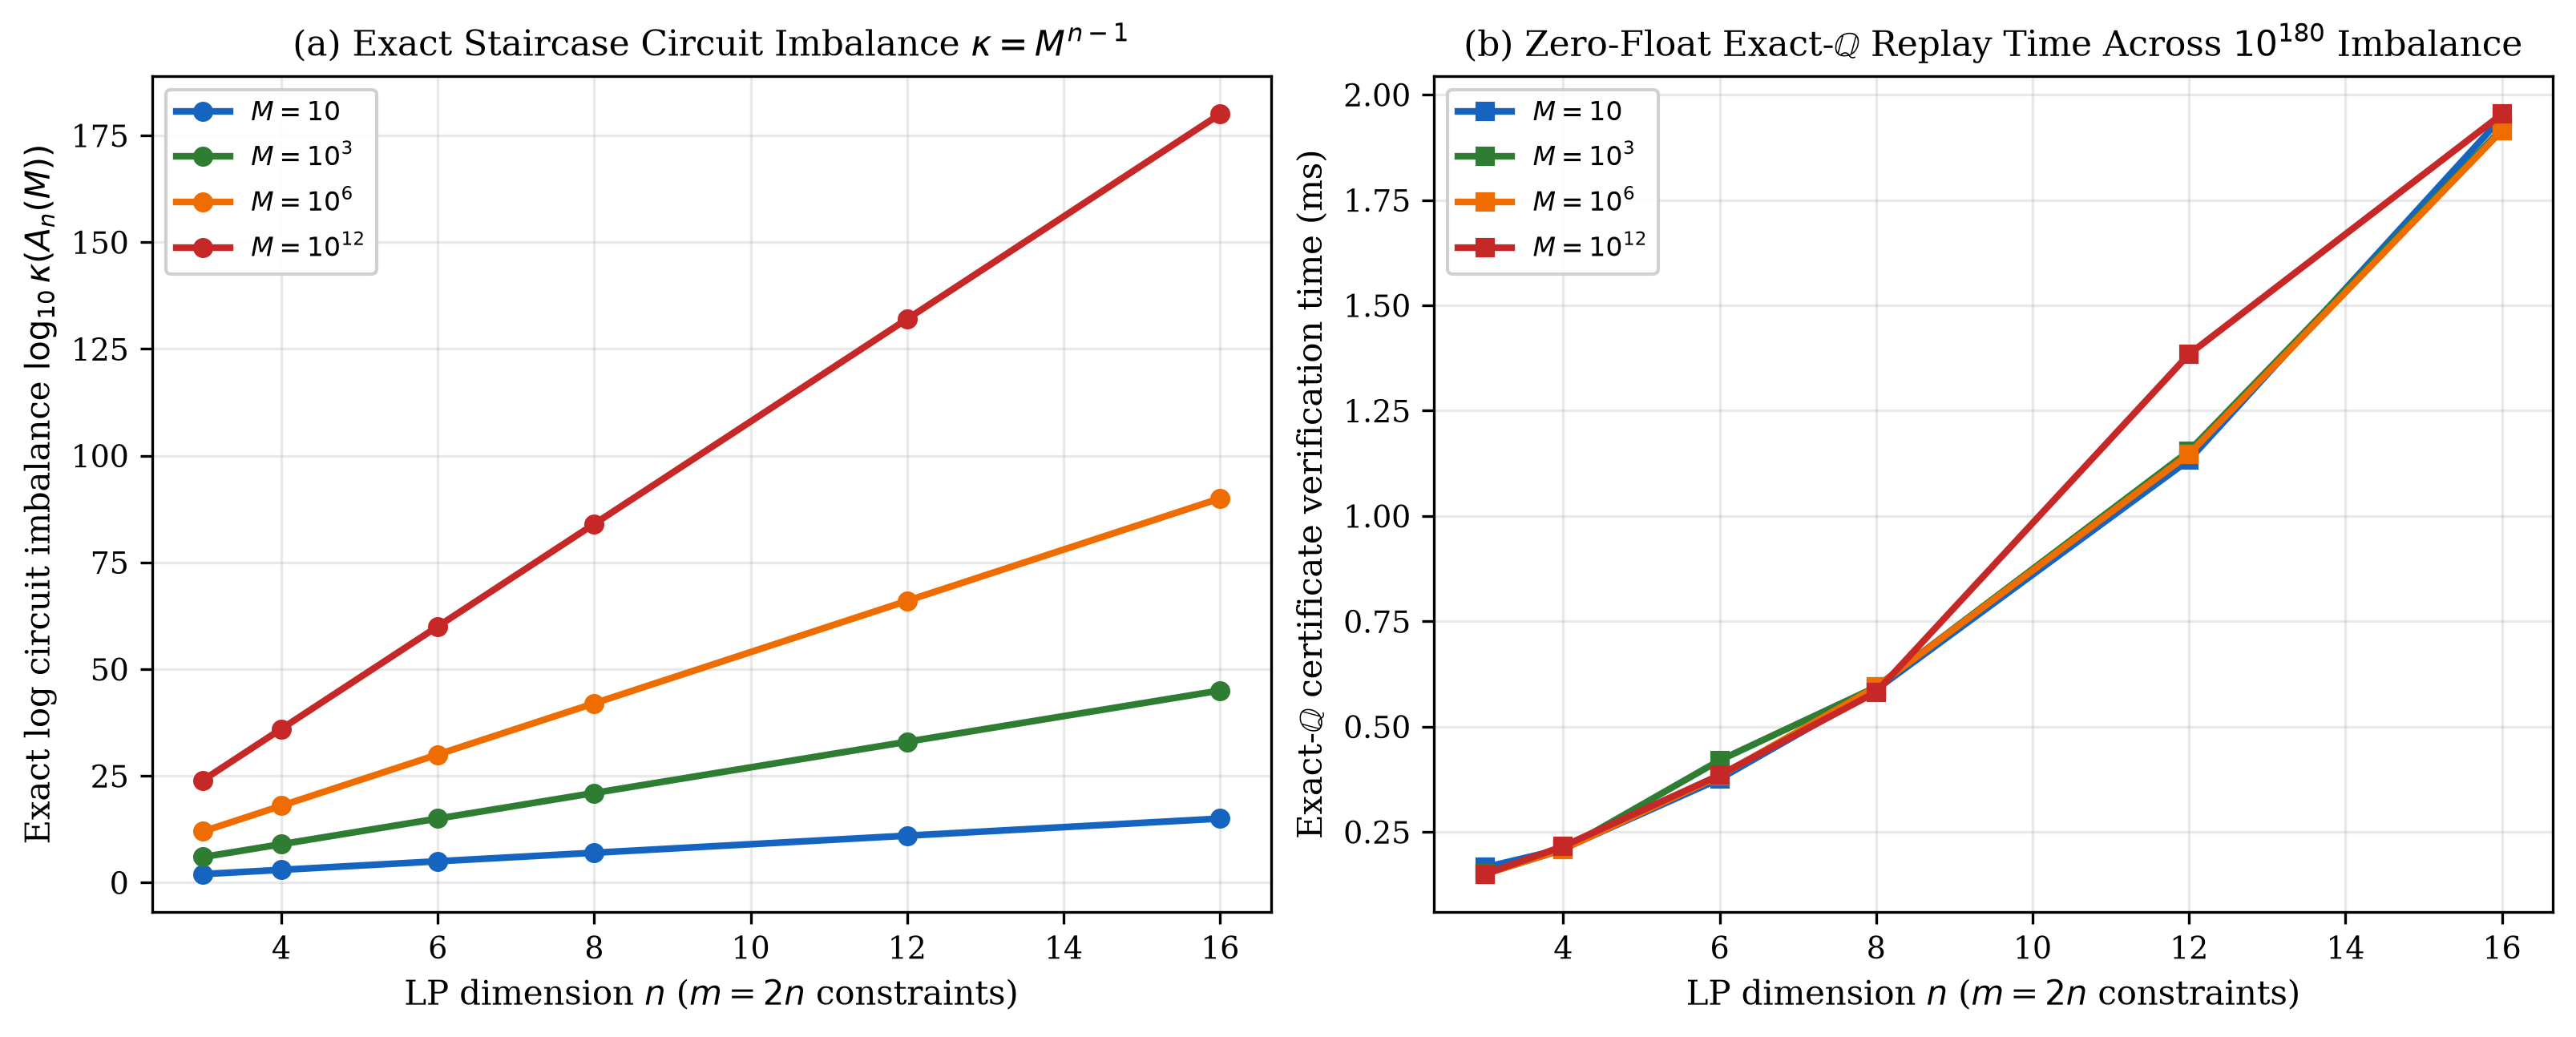
\includegraphics[width=0.95\linewidth]{figures/fig1_circuit_imbalance_scaling.png}
\caption{Staircase circuit-imbalance amplification. (a)~Exact circuit imbalance $\kappa(A_n(M)) = M^{n-1}$ growing to $10^{180}$ at $n=16, M=10^{12}$. (b)~Exact-$\QQ$ zero-float verification time remaining under $2\,\mathrm{ms}$ across all scales.}
\label{fig:imbalance}
\end{figure}

\begin{figure}[t!]
\centering
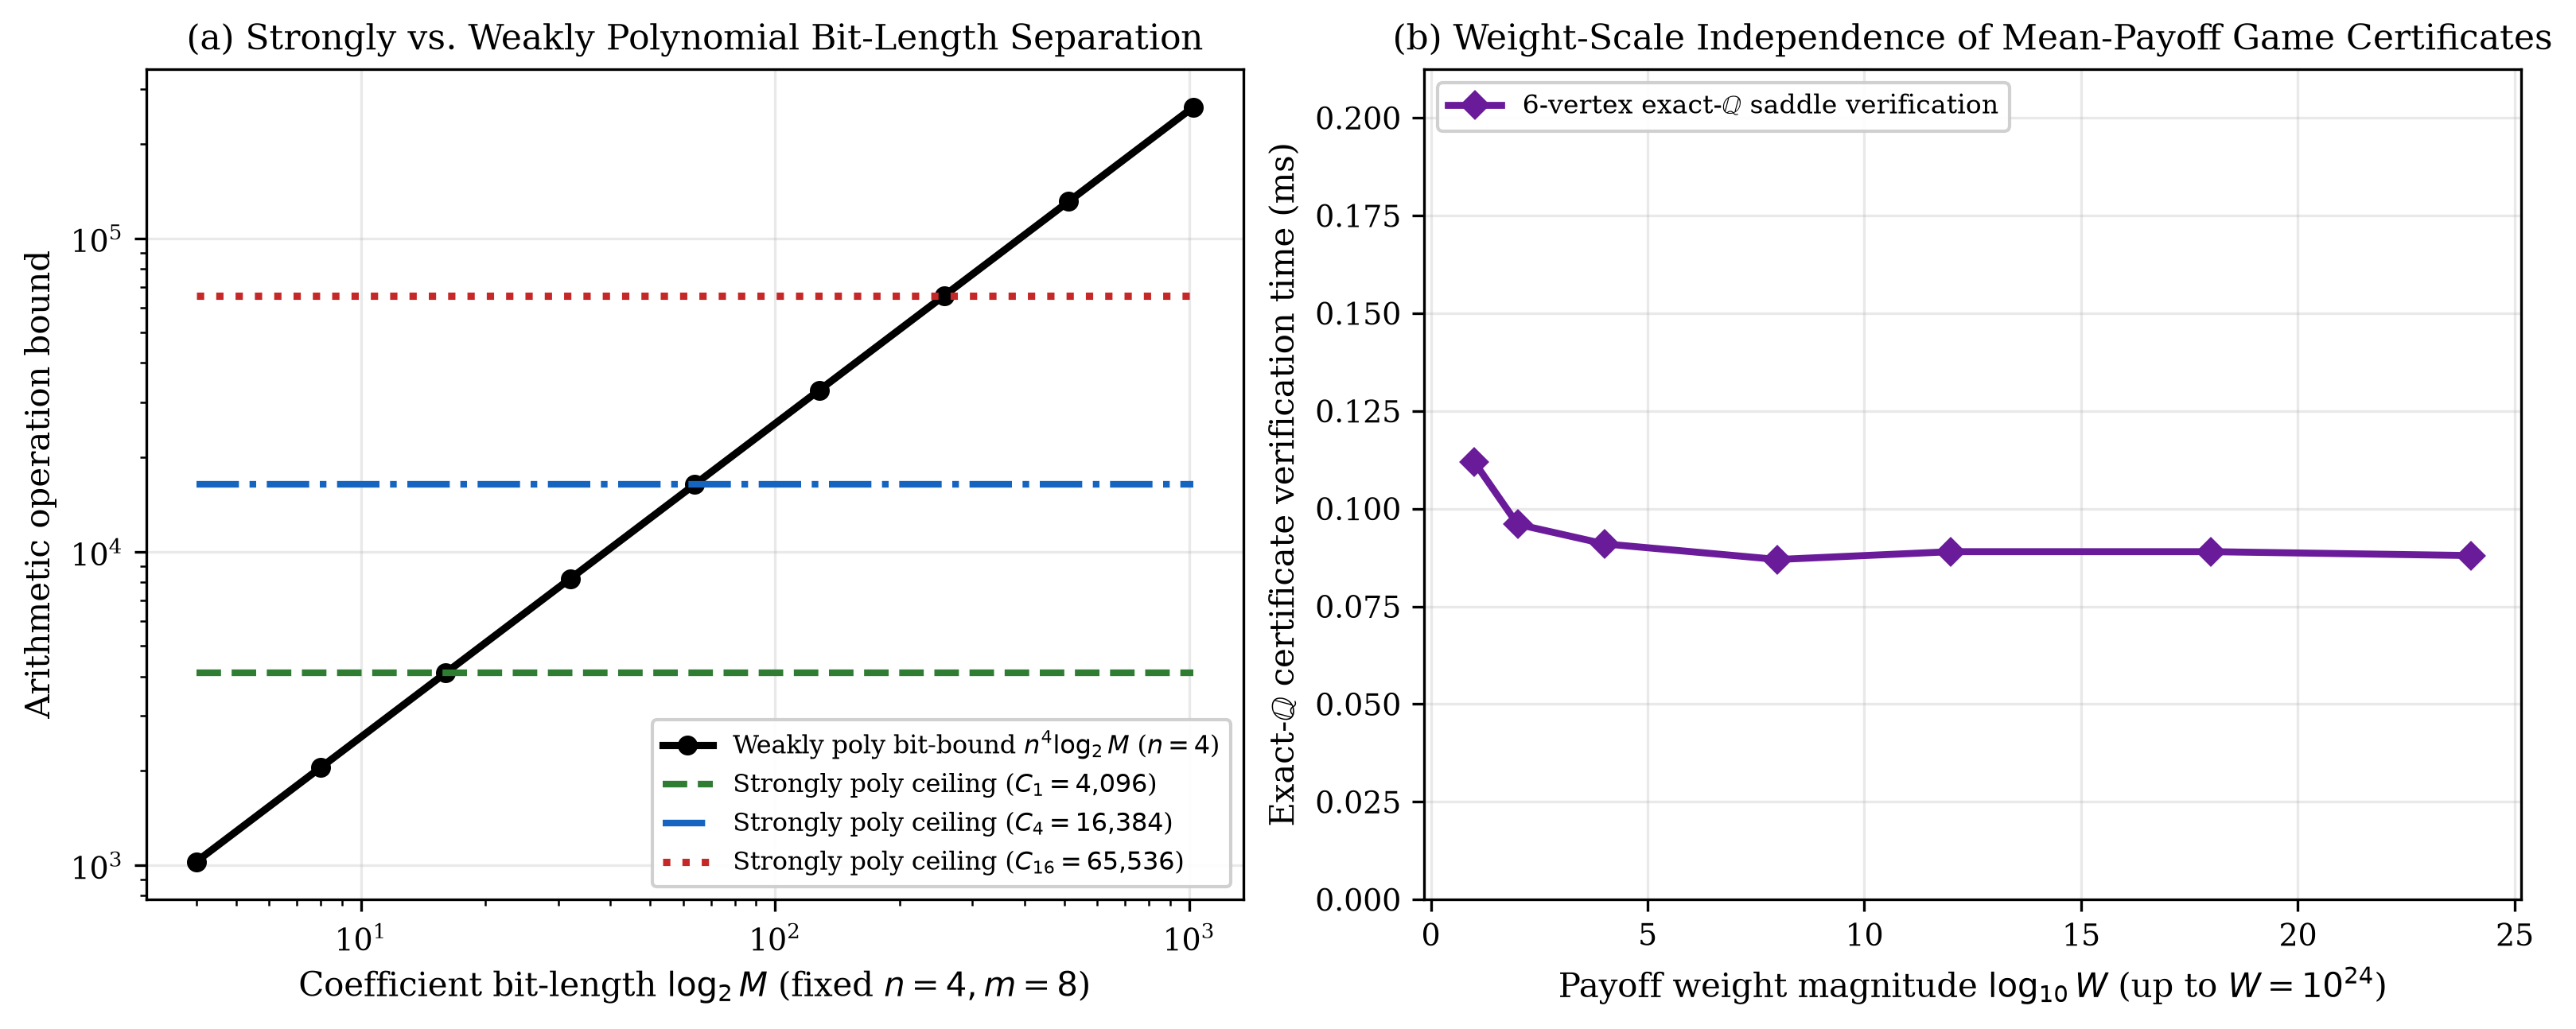
\includegraphics[width=0.95\linewidth]{figures/fig2_strongly_poly_crossover_and_mpg.png}
\caption{Bit-length separation and mean-payoff game scale invariance. (a)~Illustrative fixed-dimension ($n=4$) comparison of weakly polynomial $\log_2 M$ growth against constant strongly polynomial ceilings. (b)~Flat sub-$0.12\,\mathrm{ms}$ exact-$\QQ$ saddle verification for $6$-vertex mean-payoff games up to $W = 10^{24}$.}
\label{fig:mpg}
\end{figure}

\begin{figure}[t!]
\centering
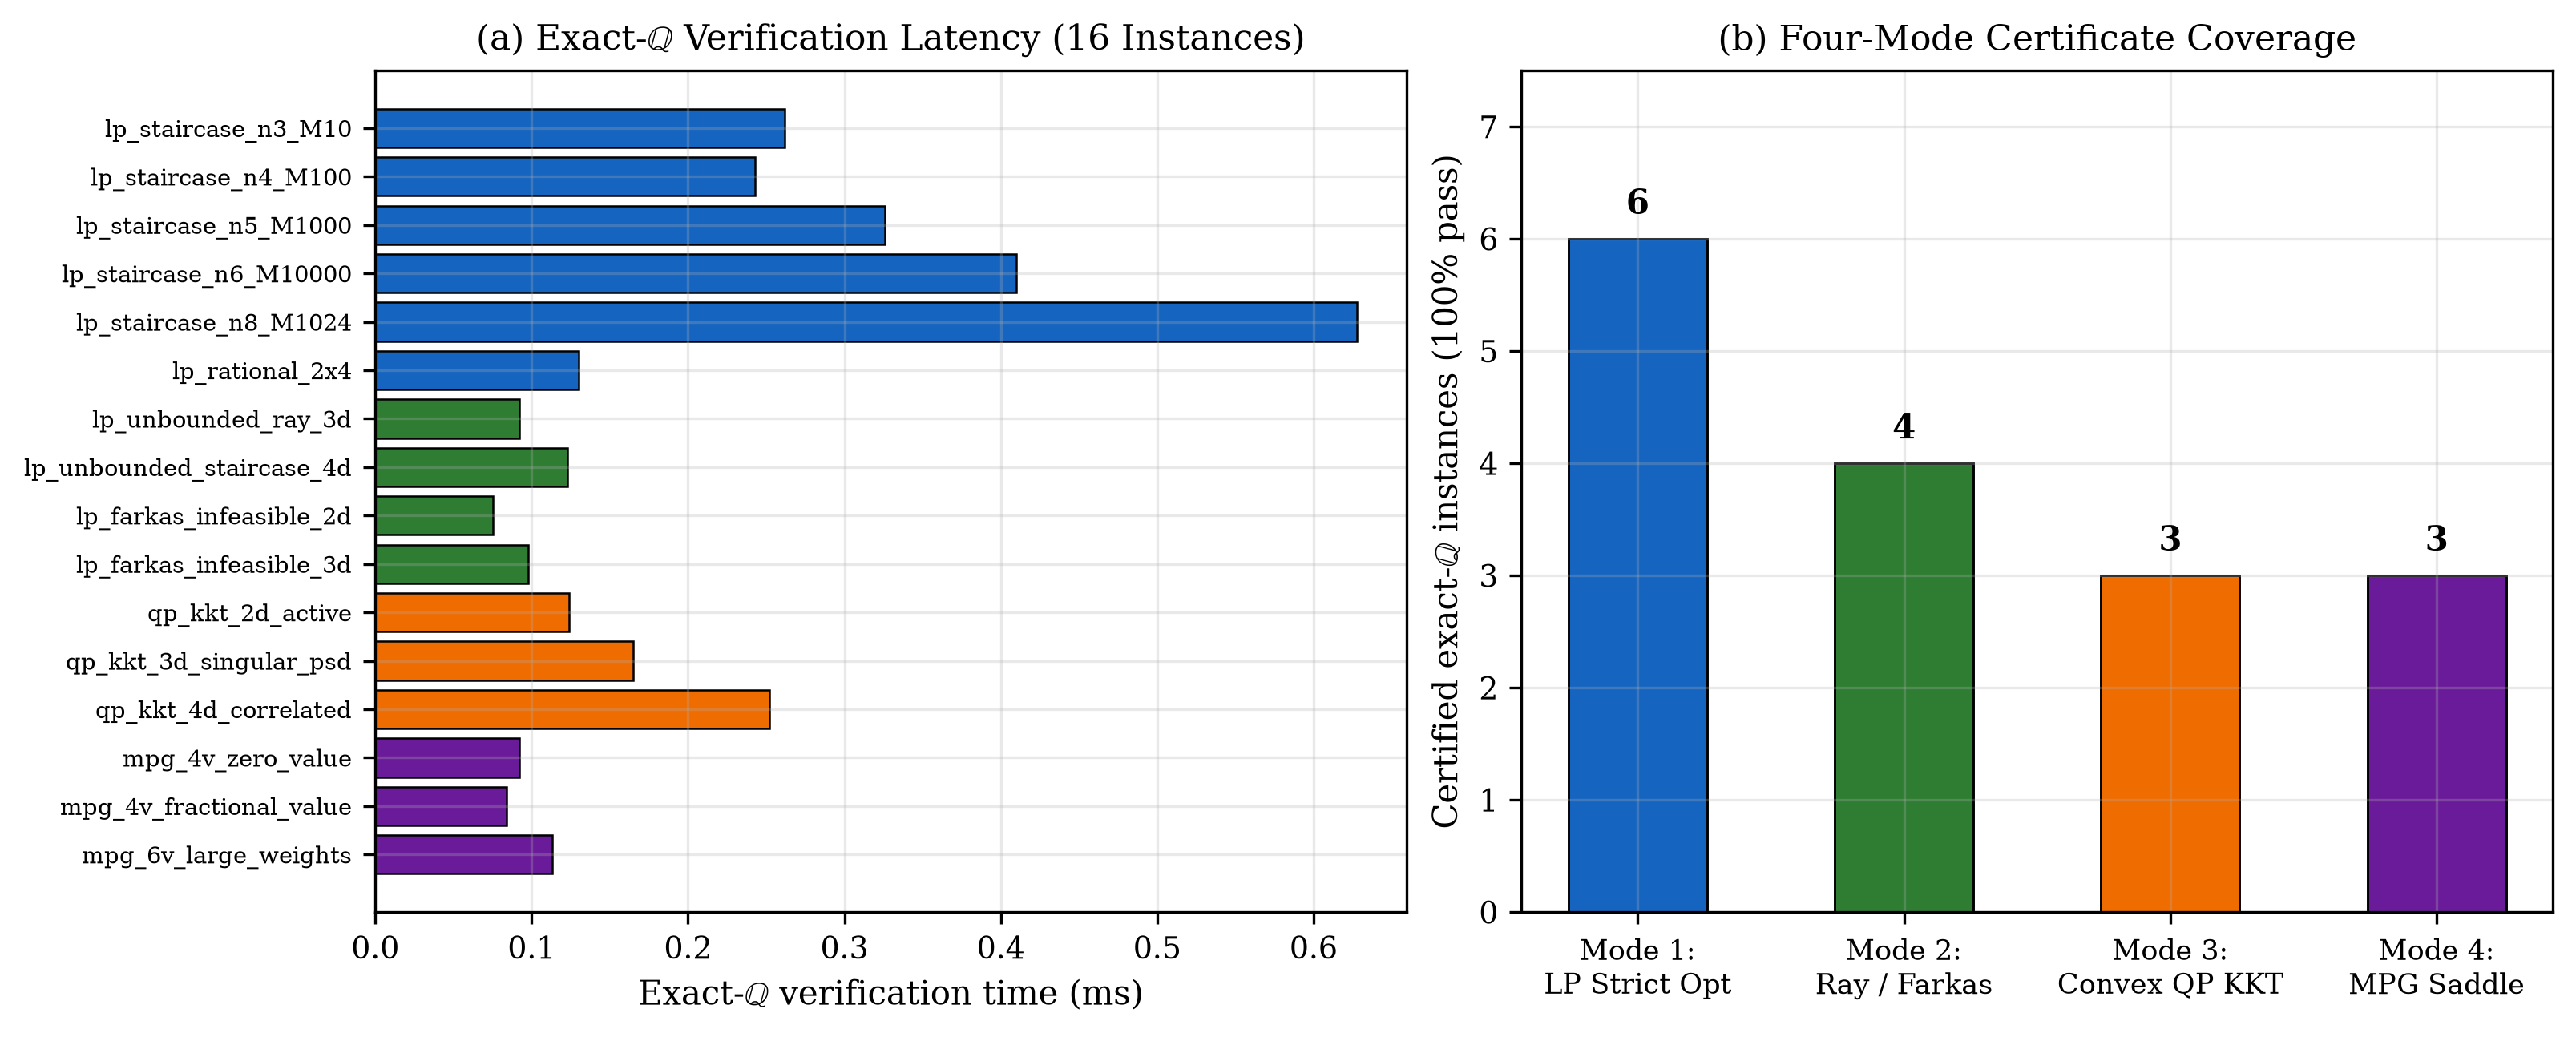
\includegraphics[width=0.95\linewidth]{figures/fig3_atlas_verification_summary.png}
\caption{Certified atlas performance. (a)~Per-instance exact-$\QQ$ verification latency across all $16$ certificates ($\le 0.63\,\mathrm{ms}$). (b)~Distribution of certified instances across OpenAI Theorem~1, Corollary~6 (convex QP), and deterministic mean-payoff games.}
\label{fig:atlas}
\end{figure}

\section{Scope Boundaries and Outlook}\label{sec:outlook}

This work certifies exact rational solver outputs rather than re-implementing OpenAI's price-rescaling search algorithm~\cite{openai2026lp}, and our Lean~4 development mechanizes the core inner-product, duality, exclusivity, price-invariance, list-vector KKT square-completion, and inductive list-cycle telescoping theorems (plus scalar scale-monotonicity Lemma~18), while delegating matrix-rank Gaussian elimination, pivoted $LDL^\top$ factorization, and graph traversal to the pure-stdlib Python verifier (\texttt{MAX\_DIM = 64}). Extending the verifier to sparse exact-$\QQ$ factorizations and stochastic mean-payoff games with rational transition probabilities is a natural next step.

\clearpage
\bibliographystyle{plain}
\bibliography{references}

\end{document}
